\chapter{Samples Explorer}

The aim of the samples explorer is to help navigate a large number of samples in a use friendly way, by dynamically generating an interface based on written rules for each sample.

\section{Working principle}

Let us assume we have a set of samples in a directory as shown in figure \ref{samples_explorer_directories}.

\def\step{0.5}
\newcommand{\dpoint}[2]{(#1*\step,-#2*\step)}
\newcommand{\dcorner}[4]{\draw [thick] \dpoint{#1}{#2} -- \dpoint{#1}{#4}; \draw [thick] \dpoint{#1}{#4} -- \dpoint{#3}{#4};}
\begin{figure}[!ht]
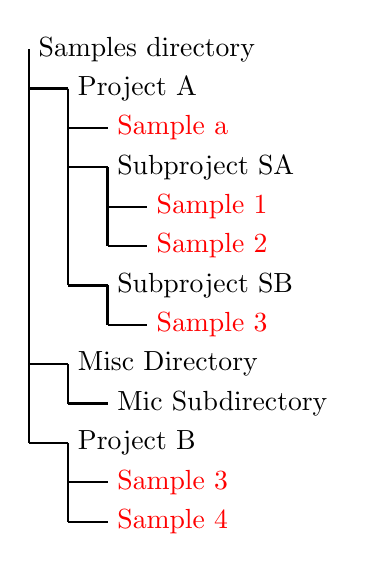
\begin{tikzpicture}
\draw (0,0) node[right]{Samples directory};
\dcorner{0}{0}{1}{1}
\draw \dpoint{1}{1} node[right]{Project A};
\dcorner{1}{1}{2}{2}
\draw \dpoint{2}{2} node[right,red]{Sample a};
\dcorner{1}{1}{2}{3}
\draw \dpoint{2}{3} node[right]{Subproject SA};
\dcorner{2}{3}{3}{4}
\draw \dpoint{3}{4} node[right,red]{Sample 1};
\dcorner{2}{3}{3}{5}
\draw \dpoint{3}{5} node[right,red]{Sample 2};
\dcorner{1}{1}{2}{6}
\draw \dpoint{2}{6} node[right]{Subproject SB};
\dcorner{2}{6}{3}{7}
\draw \dpoint{3}{7} node[right,red]{Sample 3};
\dcorner{0}{0}{1}{8}
\draw \dpoint{1}{8} node[right]{Misc Directory};
\dcorner{1}{8}{2}{9}
\draw \dpoint{2}{9} node[right]{Mic Subdirectory};
\dcorner{0}{0}{1}{10}
\draw \dpoint{1}{10} node[right]{Project B};
\dcorner{1}{10}{2}{11}
\draw \dpoint{2}{11} node[right,red]{Sample 3};
\dcorner{1}{10}{2}{12}
\draw \dpoint{2}{12} node[right,red]{Sample 4};
\end{tikzpicture}
\caption{Example of a directory tree for the samples explorer module}
\label{samples_explorer_directories}
\end{figure}
In this, the directories containing actual samples data are highlighted in red. The aim of the SE is to create a GUI that will display the chosen samples information and data, while ignoring the directories that do not have any.

To do so, the user will chose the root directory that is to be analyzed, and the program will traverse all the subdirectories looking for samples. Those are indicated by the presence of a \lsgnq{desription.txt} file inside each of them. Without one, the content of a directory will be ignored, and so will be any text file that does not match that exact file name.


\section{The description file}

As stated before, each directory of interest must contain a \lsgnq{description.txt} file. This file contains the elementary instructions that will generate the related sample user interface. Strictly speaking, it is a Lua script and will be used to call several functions.
\begin{itemize}
	\item \lfc{date}(\lsg{date in any format}) : will give a date to the sample. That date does not need to follow any particular format.
	\item \lfc{description}(\lsg{description text}) : adds a description to the sample. There is no size limit to it. New lines must be defined with a \textbackslash  n statement within the string.
	\item \lfc{tags}(\lsg{tag 1},\lsg{tag 2},\lsgnq{...}) : tags associated to the sample. They can be anything, usually project names, geometry, etc, and will be used for filtering (see \ref{samples_explorer_tags}).
	\item \lfc{add\_image}(\lsg{path}) : path to the image to display, this can be called several times to display several pictures onto the interface
	\item \lfc{image\_description}(\lsg{description text}) :  adds a description to the last image defined with \lfc{add\_image}
	\item \lfc{add\_graph}(\lsg{caption}) : defines a new graph with its associated caption
	\item \lfc{add\_data}(\lsg{first file path},\lin{column number of file 1},\lsg{second file path},\lin{column number of file 2}) : this will add data to be displayed onto the last defined graph. The data must come from text files that contains several columns. The first two arguments will define the abscissa, while the last two define the data values. Columns counting start at 0.
	 \item \lfc{axis}(\lft{x1},\lft{x2},\lft{y1},\lft{y2}) : will set the default display axis of the last defined graph
\end{itemize}
Using those functions is not mandatory, and they can be omitted if irrelevant. Here is an example of what such a file could look like:
\begin{lstlisting}
description("Sample 1")

tags("t1","t4")

add_image("im1.jpg")
image_description("First image")

add_image("im2.jpg")
image_description("Second image")

add_image("subdir/im3.jpg")

add_graph("Graph 1")
add_data("data1.txt",0,"data1.txt",1)
axis(0,10,-0.5,1.5)

add_graph("Graph 2")
add_data("data1.txt",0,"data1.txt",1)
add_data("data2.txt",0,"data2.txt",2)

add_graph("Graph 3")
add_data("data1.txt",0,"data1.txt",1)
add_data("data2.txt",0,"data2.txt",1)
add_data("data2.txt",0,"data2.txt",2)
\end{lstlisting}

\section{Interface}

Once the various samples have been put in their directories, and their description files written, using the module is fairly simple.

The very first step is to define the root directory of the samples. This is done through the \lfc{...} button within the \lfc{Directory} box. The dialog that appears will ask for the root directory.

Once set, the software browses all of the subdirectories looking for description files, and treats them. The processing can take some time depending on the number of samples. If all goes well, the interface should update in two ways:
\begin{itemize}
	\item the list on the left of the window should now be populated by a list of all the samples and their directories.
	\item the panel on the right should now contain an aggregate of all the samples, each having a sample panel.
\end{itemize}

\subsection{The sample panel}

Each sample panel contains the information specified in the associated description file. 

\subsection{Tags filtering}

\label{samples_explorer_tags}
Tags would be of little point if they could not be used to filter the results. This is the purpose of the \lfc{Filter Tags} button at the bottom left of the window. A dialog appears after clicking it, and it will help 
